\documentclass[a4paper]{book}

% Load the VUB package.
% This has many options, please read the documentation at
% https://gitlab.com/rubdos/texlive-vub
\usepackage{vub}
\usepackage{booktabs}
\usepackage{graphicx}
\usepackage{listings}
\usepackage{caption}
\usepackage{xcolor}
\usepackage{tikz}
\usetikzlibrary{arrows.meta, positioning}

\graphicspath{ {./images/} }

%\captionsetup[figure]{position=bottom}
%\captionsetup[listings]{position=bottom}


% Some highly suggested packages, please read their manuals.
%\usepackage{cleveref}
\usepackage[natbib,style=apa]{biblatex}
\addbibresource{references.bib}

\title{Distributing first-class reactors in a cluster environment}
\pretitle{\flushleft{Graduation thesis submitted in partial fulfilment of the requirements for the degree of de Ingenieurswetenschappen: Applied informatics}}
%\subtitle{Haai Virtual machine}
\author{Hans Van der Ougstraete}
\date{June~2024}
\promotors{Promotors: prof.\ dr.\ Wolfgang De Meuter,\and prof.\ dr.\ Joeri De Koster \and Supervisor: Bjarno Oeyen}

\faculty{sciences and bioengineering sciences} % Note: without the word "Faculty"!

\begin{document}
\frontmatter
\maketitle%

% Oftentimes, you need add a second language title.
\title{Distributing first-class reactors in a cluster environment}
\pretitle{\flushleft{Proefschrift ingediend met het oog op het behalen van de graad van Master of Science in de Ingenieurswetenschappen: Toegepaste informatica}}%
%\subtitle{mijn ondertitel}
\date{Juni~2024}%
\promotors{Promotors: prof.\ dr.\ Wolfgang De Meuter, \and prof.\ dr.\ Joeri De Koster \and Supervisor: Bjarno Oeyen}
\faculty{wetenschappen en bio-ingenieurswetenschappen}%
\maketitle%

\chapter{Abstract}
Reactive Programming (RP) is a powerful paradigm that models data flow as streams of events, enabling systems to react to changes and events efficiently. This document explores the principles of reactive programming, its applications, and the development of a framework for distributing first-class reactive programs in a cluster environment. We use the novel reactive language Haai, that due to its independent form (not relying on a base language) addresses key challenges in reactive programming by preventing the base language to intervene with the reactivity of the program. In this work we introduce the Haai virtual machine, implemented in Elixir, leveraging the Erlang Virtual Machine (BEAM) to enable the distribution of reactive programs across a cluster.

The evaluation of the cluster environment demonstrates its flexibility, scalability, and fault tolerance, allowing for the simulation of large cluster environments. A practical use case, the distributed reactive melody generator, showcases the framework's application in transforming streams of data into synthesized sound by sending network messages to a Supercollider sound server. This use case highlights the potential of reactive programming in creating innovative and dynamic systems that respond to real-time events. Overall, this work contributes to the advancement of reactive programming by providing a robust framework for distributed reactive programming and demonstrating its practical applications in a musical context.

\tableofcontents%

\mainmatter%
\chapter{Introduction}

Reactive Programming (RP) represents a broad programming paradigm centered around responding to changes and events within a system. This paradigm involves modeling data flow as streams of events and utilizing declarative and composable abstractions to manage asynchronous and event-driven scenarios. The canonical reactive program model, often exemplified by spreadsheets, is based on time-varying values and the propagation of change. 

The choice of reactive programming is motivated by several key advantages. Firstly, RP enables systems to respond quickly to changes in data and events, making it ideal for real-time applications. Secondly, reactive systems can scale up or down based on demand, allowing for efficient resource utilization and adaptability to varying loads. Thirdly, the event-driven nature of reactive programming facilitates communication between components through messages, promoting modular design with a minimal dependency between modules (loose coupling). Finally, reactive programming encourages the use of declarative constructs, which can lead to more readable and maintainable code. Composable abstractions allow for the creation of complex behaviors from simple building blocks.

This document delves into the intricacies of reactive programming, its applications, and the development of a framework to experiment with the distribution of first-class reactors in a cluster environment. We also present a practical use case involving a sound-generating instrument that reacts to numerical input and delivers values to a sound-generating server.

The canonical reactive program model (\cite{DBLP:journals/csur/BainomugishaCCMM13}) is based on time-varying values and propagation of change. Spreadsheets offer a good example to illustrate this. When a cell containing a formula that includes other cells it is dependent on the cells that are used in that formula. As an example lets take a cell A3 that contains the formula "=A1*A2" whenever the value changes in the cells A1 or A2, A3 will automatically update. We call each spreadsheet cell a time-varying value or signal because there concrete value changes over time due to events. In this example, an event could be when a user changes the value A1 or A2 using the gui of the spreadsheet program.

The two fundamental abstractions defined by RP to represent time-varying values are behaviors and events. Behaviors have a value at any moment (continuous) and events have a value at specific moments in time (discrete). 
Listing \ref{code:Haairp} shows the spreadsheet example represented in the RP language Haai (\cite{oeyen_reactive_2024}).
In this example a3 is defined as a reactor that continuously contains the result of a1 * a2. For each time that an event occurs updating a1 or a2, a3 will be automatically updated. 

\newpage

\begin{lstlisting}[language=C, caption={Haai code}, captionpos=b, label={code:Haairp}, basicstyle=\ttfamily, frame=single]
	(defr a3 (* a1 a2))
\end{lstlisting}

The updates to a3 occur in such a way that the value for a3, which could be a dependency to another cell in the spreadsheet, is always correct or updated such that there are no invalid or intermediary values. The rhythm of the propagation of change for reactor a3 depends on the speed that events occur. Figure \ref{fig:a3} shows the value for reactor a3 (* a1 a2) over time presenting three updates t=0, t=1 and t=2. 

Reactor a3 is an example of a small reactive program. Multiple reactors can be combined in a bigger reactive program resulting in a reactor composed out of reactors. If our system is constructed solely from reactors we call this a purely reactive program since reactors serve as the only building blocks.


\begin{figure}[h]
	\centering
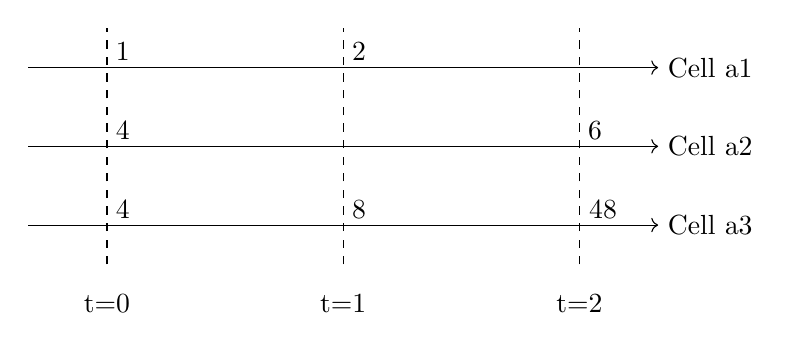
\begin{tikzpicture}[node distance=1cm]
	% Define the variables and their values at different times
	\node (A1) at (0.2, 2.2) {1};
	\node (A2) at (3.2, 2.2) {2};
%	\node (A3) at (6, 2) {a1: 3};
	
	\node (B1) at (0.2, 1.2) {4};
%	\node (B2) at (3, 1) {B: 5};
	\node (B3) at (6.2, 1.2) {6};
	
	\node (C1) at (0.2, 0.2) {4};
	\node (C2) at (3.2, 0.2) {8};
	\node (C3) at (6.3, 0.2) {48};
	
	% Draw the horizontal lines
	\draw[->] (-1, 2) -- (7, 2) node[right] {Cell a1};
	\draw[->] (-1, 1) -- (7, 1) node[right] {Cell a2};
	\draw[->] (-1, 0) -- (7, 0) node[right] {Cell a3};
	
	% Draw the vertical lines to indicate the same moment in time
	\draw[dashed] (0, -0.5) -- (0, 2.5);
	\draw[dashed] (3, -0.5) -- (3, 2.5);
	\draw[dashed] (6, -0.5) -- (6, 2.5);
	
	% Label the moments in time
	\node at (0, -1) {t=0};
	\node at (3, -1) {t=1};
	\node at (6, -1) {t=2};
\end{tikzpicture}
    \caption{Timeline of cells a1, a2 and a3 over time.}
\label{fig:a3}
\end{figure}
     


\section{Problem Statement}
To our best knowledge we did not find a framework to experiment with the distribution of first-class reactors. We developed a framework to study the distribution of first-class reactors in a cluster environment and create a declarative specification to deploy a distributed reactive program into different cluster environments. To show the working state of the framework we deployed a sound generating instrument that reacts on input and delivers values to be send to a sound generating server.  

\section{Structure of the Thesis}
We first look at non-reactive programming and distributed reactive programming in section \ref{sec:rp}. Chapter \ref{sec:distribution} explains the distribution of the runtime and the tools used to build it. After the evaluation of the distribution framework and the musical use case of the distributed reactive melody generator in section \ref{sec:evaluation} we conclude. 


\chapter{Reactive Programming} \label{sec:rp}

Reactive programming (RP) and reactive streams (RS) are terms that are often used interchangeably. Both adhere to the same canonical model.  For as much as they have in common there are two fundamental differences, the way dependencies between signals are established and how updates to signals are orchestrated.

\subsubsection{Signal Dependencies}
The way signal dependencies are established in the source code differs in the following way. In RP languages these dependencies are automatically taken care of by the language. Programmers implement there desired functionality in RP similar as they would in a non-reactive language. In RS the dependencies are explicitly programmed by the programmer by making use of operators provided by the RS library. The programmer creates a linear application of those operators often called a pipe as shown in listing \ref{code:rxpy}, where an observable existing of the numbers 1 to 10 will be the source of the pipe. The second or last operator in the pipe is Sum, who will produce one value to be printed on screen.

\subsubsection{Signal Orchestration}
The operators used in RS define independently for each signal how these will be updated. In contrary to RP where it is again the system that updates signals in a global way. As can be seen in listing \ref{code:Haairp}, no special code defines how or in what order the values a1 and a2 need to be updated. Both approaches can fail and result in inconsistencies in the values, if for example the RP language updates signals in the wrong order, dependent signals end up having the wrong value, this is called a glitch. On the other hand in RS, if the programmer does not exactly know what an operator does and uses it in a pipe or collection of operators, inconsistencies might arise and also produce a glitch. 

\vspace{1em} % Adjust the space as needed
\noindent
The responsibility to handle signal dependencies and orchestration correct is at the system side for RP and in the developers hand for RS.


\begin{lstlisting}[language=Python, caption={Python, RxPy library},captionpos=b, label={code:rxpy}, basicstyle=\small\ttfamily, frame=single]
rx.of(1,2,3,4,5,6,7,8,9,10).pipe(
	operators.filter(lambda i: i %2 == 0),
	operators.sum()
).subscribe(lambda x: print("Value is {0}".format(x)))
\end{lstlisting}


\section{State-of-the-Art}

\subsection{non-Distributed Reactive Programming}
Reactive programming has many applications, here we will show three selected examples. Fran (\cite{DBLP:conf/icfp/ElliottH97}) the first reactive programming language, originated to compose interactive multimedia animations based on behaviors and events. Listing \ref{code:fran} show a small fran code example that animates a bitmap file with the moveXY behavior given the argument wiggle (a value that changes over time form 0 to +1 to -1 back to 0 and so on) for x and 0 for y.
\begin{lstlisting}[language=Python, caption={Fran, animation (\cite{DrDobb})},captionpos=b, label={code:fran}, basicstyle=\small\ttfamily, frame=single]
leftRightCharlotte = moveXY wiggle 0 charlotte
charlotte = importBitmap "../Media/charlotte.bmp"
\end{lstlisting}

ReactiFi (\cite{DBLP:journals/programming/SterzEMBGHMF21}) a high-level reactive programming language to program Wi-Fi chips on mobile consumer devices without expert knowledge of Wi-Fi chips. In listing \ref{code:reactifi} we show part of the code for adaptive file sharing programmed on the Wi-Fi chip. A ReactiFi program exists out of reactives, like monitor, frames en count in the example. Reactives are reactive definitions of individual processing steps that are triggered by incoming events. The source are wifi frames gathered in 'monitor' mode. Those frames are filtered for a certain address ADDR and summed in the last step (count) of the example.

\begin{lstlisting}[language=Python, caption={ReactiFi, Wi-Fi file sharing (\cite{DBLP:journals/programming/SterzEMBGHMF21})},captionpos=b, label={code:reactifi}, basicstyle=\small\ttfamily, frame=single]
 val monitor = Source(Monitor)
 val frames  = monitor.filter(frame -> { frame.dst == ADDR })
 val count   = frames.fold({ 0 })((count, frame) -> { count + 1 })
\end{lstlisting}

The domain-specific language Yampa (\cite{DBLP:conf/haskell/CourtneyNP03}) embedded in Haskell for programming hybrid (mixed discrete-time and continuous-time) systems. n Yampa, a signaling function (SF) is a fundamental concept that represents a continuous-time signal transformer. An SF takes an input signal and produces an output signal over time. Signaling functions are the basic building blocks of Yampa programs and are used to model and manipulate continuous-time behaviors. Listening \ref{code:yampa} shows such a signal function named fallingBall. This SF describes the behavior of a bouncing ball with a position (p) and velocity (v). When the discrete event 'hitGround' occurs the velocity of the ball reverses to simulate the bounce of the ball.
\begin{lstlisting}[language=Python, caption={Yampa, bouncing ball (\cite{YampaBook})},captionpos=b, label={code:yampa}, basicstyle=\small\ttfamily, frame=single]
-- The bouncing ball signal function
fallingBall :: SF () Ball
fallingBall = proc () -> do
 rec
   -- Velocity integrates to position
   v <- integral -< gravity
   p <- integral -< v

   -- Event that occurs when the ball hits the ground
   let hitGround = if p <= 0 then Event () else NoEvent
	
   -- Velocity changes direction on hit
   v <- (arr (\v -> if p <= 0 then -v else v) <<< identity) -< v

 returnA -< (p, v)
\end{lstlisting}


Most, if not all, of the reactive programming languages are build on top of a sequential host language. Fran and Yampa are build on Haskell, ReactiFi is build on Scala and C. This allows the reactive programming languages to leverage the existing ecosystems of the host language. For example a host languages can provide functions to be called form the reactive programming language, this is called lifting, the host-functionality is lifted form the host language into the RP language adapted to work with continuous and discrete notions of time. On the other hand, when a system is composed of those two components, the host part and the reactive part, they are prone to the \textit{Reactive Thread Hijacking Problem} and the \textit{Reactive/Imperative Impedance Mismatch} problems (\cite{vonder_tackling_2020}). Both problems might turn the reactive program nonreactive. In the first case the event-handling logic could block the main thread of execution, preventing other events from being processed on time. Secondly reactive and imperative paradigms have fundamentally different ways of handling state and flow, which can lead to error-prone code. In section \ref{sec:prp} we will introduce a novel reactive language Haai that by design excludes both problems mentioned above. This will help us in distributing the reactors since both problems will not arise by design.  


\subsection{Distributed Reactive Programming} \label{sec:drp}


Many distributed systems can be seen as some kind of reactive system. For example an internet of things application with many connected sensors that feed information into a reactive system. Or a distributed reactive system with strong computational differences for different behaviors that should finish in a bounded time. The distribution can optimize the placement of code with respect to different computational capacities related to the application. 

Once working in a distributed setting, typical problems arise like data inconsistencies and node disconnects and crashes. n the RP literature, inconsistencies in the data are called glitches. A glitch is a momentary inconsistency in a time-varying value. For instance, consider a distributed reactive system that monitors the temperature of a network of sensors. Each sensor reports its temperature reading to a central processing unit, which then calculates the average temperature across all sensors. If one sensor temporarily malfunctions and reports an incorrect temperature, this erroneous value can introduce a glitch into the system. The central processing unit may briefly calculate an inaccurate average temperature based on the faulty data, leading to a momentary inconsistency. However, once the sensor corrects its reading or is identified as faulty, the system can recover and resume providing accurate temperature information. Being free of glitches is called glitch-freedom (\cite{DBLP:journals/tse/MargaraS18}). 

As an example we show REScala. Built on top of the Scala programming language. The framework introduces several core concepts, including signals, events, and signal functions. Signals represent time-varying values that model the state of a system over time, while events are discrete occurrences that trigger changes in signals or other events. Signal functions, also known as signal transformers, take one or more signals as input and produce one or more signals as output, enabling the transformation, combination, or filtering of signals. ReScala provides a flexible and efficient way to build reactive systems, making it well-suited for applications ranging from real-time data processing to interactive user interfaces. Listing \ref{code:rescala} shows a small example where the program prints the actual time + 1000ms for 5 seconds. The observe method is used to receive and print the value in side the offsetSignal.

\newpage

\begin{lstlisting}[language=Scala, caption={REScala, time + 1000},captionpos=b, label={code:rescala}, basicstyle=\small\ttfamily, frame=single]
object ReScalaExample extends App
{
	// Define a signal that represents the current time
	val timeSignal = Signal { System.currentTimeMillis() }
		
	// Adds a constant value to the time signal
	val offsetSignal = timeSignal.map(_ + 1000)
		
	// Print the current value of the offset signal
	offsetSignal.observe(println)
		
	// Keep the application running
	Thread.sleep(5000)
}
\end{lstlisting}

 Regarding to distribution ReScala provides a solution to node disconnects and crashes in distributed reactive programs. REScala does not delegate the responsibility to handle errors to the host language (Scala). REScala has been extended to support recovery after node crashes and cope with unreliable network connections by enhancing the data flow graph for a particular program (\cite{DBLP:conf/ecoop/MogkBSFM18}). Listing \ref{code:rescala} shows a shared calendar application written in REScala. This is a distributed application where one calendar is shared among many users. In order to provide recovery after crashes, signals such as \texttt{Var[Date]} are stored in snapshots. This allows for the signal to be reloaded after a crash. In cases where a signal is dependent on dynamic signals in the network of distribution, the REScala program handles errors explicitly. For example the selectedEntries in code listing \ref{code:distrescala} expects a value from another node (selectedWeek.value). The \texttt{try catch} block will by default wait for the value but by returning false in the catch block the filter will drop this signal and continue filtering when a 'disconnectedSignal' error is received. By doing so the program does not block and keeps on running reactively.  
 
\newpage

\begin{lstlisting}[language=Scala, caption={REScala, shared calendar application, (\cite{DBLP:conf/ecoop/MogkBSFM18})},captionpos=b, label={code:distrescala}, basicstyle=\small\ttfamily, frame=single]
val newEntry = Evt[Entry]()
val automaticEntries: Event[Entry] = App.nationalHolidays() 
val allEntries = newEntry || automaticEntries 

val selectedDay: Var[Date] = Var(Date.today) 
val selectedWeek = Signal { Week.of(selectedDay.value) } 

val entrySet: Signal[Set[Entry]] = 
 if (distribute) ReplicatedSet("SharedEntries").collect(allEntries)
 else allEntries.fold(Set.empty) { (entries, entry) => entries + entry}

case class Entry(title: Signal[String], date: Signal[Date]) 

val selectedEntries = Signal {
 entrySet.value.filter { entry => 
 	try selectedWeek.value == Week.of(entry.date.value)
 	catch { case DisconnectedSignal => false } 
 } 
} 

allEntries.observe(Log.appendEntry)
selectedEntries.observe(
 onValue = Ui.displayEntryList, 
 onError = Ui.displayError)
\end{lstlisting}


\section{Purely reactive programming} \label{sec:prp}
In all previous examples the reactive programming language is build on top of a host language that lend some functionality to the reactive program. What we will discuss next is the idea of a purely reactive program. A reactive program constructed by combining only reactive programs that we call reactors.
\subsection{Reactors}
In Haai, a purely reactive computer language, the only construct available for expressing computations is a reactor. A reactor is a sort of blue print (as shown in figure \ref{fig:reactor}) that will be used to deploy any number of deployments based on that reactor. 

This blue print holds the following information: a name, number of sources, number of sinks and two types of instructions. Deployment-time instructions to be run at deployment time and reaction-time instructions that will loop over and over once the reactor is deployed. 

We can write a single reactor or combine multiple reactors in one composed reactor or reactive program. A composed reactor is build solely out of reactors, these can be native or user defined. Every computation in a pure RP program is done by a reactor, some are native to the runtime others are user defined. For example the runtime could provide native reactors for basic arithmetic. All functionality in the purely reactive programming language Haai comes from the language itself, it is not build on top of a general-purpose host language. 

\begin{figure}[h]
	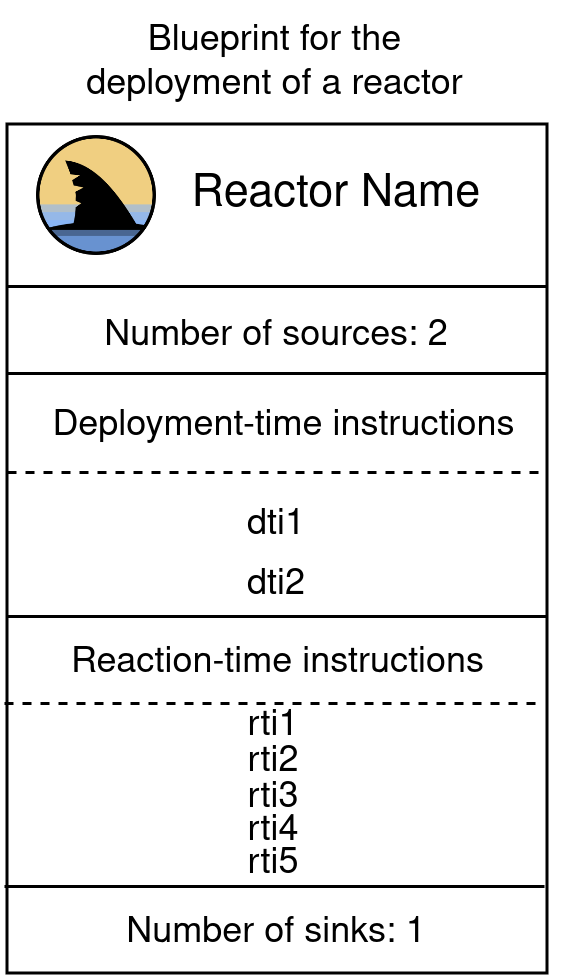
\includegraphics[scale=0.2]{reactor300.drawio}
	\centering
	\caption{Graphical representation of a reactor}
	\label{fig:reactor}
\end{figure}

The deployment of a reactor reacts on a data stream, that data altered by the reaction is found in the sink of the reactor. The deployment of a reactor is further explained in section \ref{sec:dar}.

\subsection{Haai}
We make use of the novel purely reactive language Haai. Haai is reactive all-the-way-trough. As such the only construct available for expressing computations is a reactor. A reactor has sources or inputs and sinks or outputs. For each time the sources are updated the reactor will react and produce a new sink value. The number of sources and sinks are variable per reactor definition. In Haai there are no functions, only reactors. This allows us to build reactive programs without functions (\cite{oeyen_reactive_2024}). Haai is an independent language, it does not work on top of a host-language.  

Listing \ref{code:Haai} represents three user defined reactors: consonance, duration and main. The main reactor is build out of the two user defined reactors consonance and duration and makes no use of native reactors (except for the ones in consonance and duration). Consonance and duration make use of multiple native reactors to perform arithmetic. The arguments to the reactor are the sources and the keyword 'out' defines the sink of the reactor.

\begin{lstlisting}[language=C, caption={Haai code}, captionpos=b,label={code:Haai}, basicstyle=\ttfamily, frame=single]
(defr (consonance f)
	(out (* ci f)))

(defr (duration bpm)
	(def q (/ 60000 bpm))
	(out (* lm q)))

(defr (main f bpm)
	(out (consonance f))
	(out (note_length bpm)))
	
\end{lstlisting}
The reactor in listing \ref{code:Haai} has two sources (f and bpm) and two sinks defined with the keyword out. To port the Haai code (listing \ref{code:Haai}) into the cluster environment we compile the Haai code into a byte code representation (listing \ref{code:bytecode}) that was developed for the Remus virtual machine. "a virtual machine that has been carefully designed for resource constrained computing environments."(\cite{oeyen_remus_2022})


\subsection*{Remus Instruction Set}
The Remus instruction set in table \ref{tab:instructionset} is the set of low-level operations that the virtual machine can execute. A Haai program or Reactor will after compilation exist out of a combination of instructions. Instructions form the Remus instruction set as listed here under. The Haai virtual machine is an implementation of this instruction set in Elixir. The following example program is build up out of a combination of the Remus instruction set. It is the compilation of the main reactor shown in the code snippet above. 

\begin{table}[h!]
	\centering
	\begin{tabular}{@{}lll@{}}
		\toprule
		\textbf{Instruction} & \textbf{Arguments} & \textbf{Description} \\ \midrule
		I-ALLOCMONO & [reactor]  & Allocate memory for the given reactor. \\
		I-LOOKUP & [signal]  & Lookup the value for signal \\
		I-SUPPLY & [from, destination, index] &  Move a value.\\
		I-REACT  &[memory\_location] & Apply the reaction found in memory. \\
		I-CONSUME & [memory\_location, index] & Position the result of react in run-time-memory. \\
		I-SINK & [rti\_location, sink\_index]& Position a value from run-time-memory into sink. \\ 
		\toprule
	\end{tabular}
	\caption{Remus instruction Set (\cite{oeyen_remus_2022})}
	\label{tab:instructionset}
\end{table}

\newpage

\subsubsection*{Bytecode example}

In listing \ref{code:bytecode} we show compiled Haai code from listing \ref{code:Haai}. In this bytecode example based on the Remus instruction set we see two user defined reactors named consonance and note\_length followed by the main reactor with 2 sources and 2 sinks that represents the actual reactive program that will be deployed in the cluster environment.

\begin{lstlisting}[language=C, caption={Remus bytecode as Elixir nested lists},captionpos=b, label={code:bytecode}, basicstyle=\ttfamily\footnotesize, frame=single]
[
 [:consonance, 1, 1,
	[
		["I-ALLOCMONO", :multiply]
	],
	[
		["I-LOOKUP", :ci],
		["I-SUPPLY",["%RREF",1],["%DREF",1],1],
		["I-SUPPLY",["%SRC",1],["%DREF",1],2],
		["I-REACT",["%DREF",1]],
		["I-CONSUME",["%DREF",1],1],
		["I-SINK",["%RREF",5],1]]
	],

 [:duration, 1, 1,
	[
		["I-ALLOCMONO", :divide],
		["I-ALLOCMONO", :multiply]
	],
	[
		["I-SUPPLY",60000,["%DREF",1],1],
		["I-SUPPLY",["%SRC",1],["%DREF",1],2],
		["I-REACT",["%DREF",1]],
		["I-LOOKUP",:lm],
		["I-SUPPLY",["%RREF",4],["%DREF",2],1],
		["I-CONSUME",["%DREF",1],1],
		["I-SUPPLY",["%RREF",6],["%DREF",2],2],
		["I-REACT",["%DREF",2]],
		["I-CONSUME",["%DREF",2],1],
		["I-SINK",["%RREF",9],1]]
	],

 [:main, 2, 2,
	[
		["I-ALLOCMONO", :consonance],
		["I-ALLOCMONO", :note_length]
	],
	[
		["I-SUPPLY",["%SRC",1],["%DREF",1],1],
		["I-REACT",["%DREF",1]],
		["I-SUPPLY",["%SRC",2],["%DREF",2],1],
		["I-REACT",["%DREF",2]],
		["I-CONSUME",["%DREF",1],1],
		["I-SINK",["%RREF",5],1],
		["I-CONSUME",["%DREF",2],1],
		["I-SINK",["%RREF",7],2]
	]
 ]
]
\end{lstlisting}

\section{Haai virtual machine} \label{sec:Hvm}
To run the Haai code (compiled into bytecode) we implement in this thesis a virtual machine for Haai. Implementing a virtual machine (VM) to run a new programming language offers several compelling advantages. A VM provides a layer of abstraction that insulates the language from the underlying hardware, ensuring portability across different platforms. The VM manages the memory and can be used to facilitate the implementation of advanced language features. 

The purpose of the Haai virtual machine (Hvm) is to enable the distribution of first-class reactor Haai programs in a cluster environment. The Hvm is developed in Elixir, a programming language know for its powerful features in terms of distribution and concurrency. It leverages the Erlang Virtual Machine (BEAM), which is renowned for its ability to build scalable, fault-tolerant, and distributed systems (\cite{10.5555/1951582}).

\subsection{Deploying a Reactor} \label{sec:dar}
A reactor can be seen as a blueprint for its deployment, similar to how an object created from a class in object-oriented programming is an instantiation of the blueprint that the class represents. The deployment of the reactor will request a certain size of memory. 
That total block of memory (shown in figure \ref{fig:rde}) on the right side of the reactor exists out of four main parts: sources, deployment-time memory (dtm), reaction-time memory (rtm) and the sinks. 

When we go from a reactor to a deployment we can find the following information in the reactor or blueprint for the deployment: the number of sources and sinks, the deployment time instructions (dti) and the reaction time instructions (rti). For each source and each sink a position is reserved in the memory. Based on the deployment-time instructions defined in the reactor we can prepare the deployment-time memory (dtm). This deployment-time memory part of the full memory block will reserve space for the deployment of the reactors found in the dti. The dtm size is defined upfront by matching the deployment time instructions that will be executed once, when the reactor is deployed. 

The full memory block is almost allocated, the space for the sources, the sinks and dtm has been reserved, the last step is to reserve space for the reaction-time memory (rtm). The space required for rtm is equal to the number of instructions found in the reaction time instructions (rti). For each instruction in rti there is one block reserved in rtm. A deployed reactor uses the four memory parts: sources, dtm, rtm and sinks to react according to the reaction-time instructions found in rti. Knowing the index of the rti instruction that is executed is primordial, since we based the implementation around this index. The index of an instruction relates directly to a location in memory. 

\begin{figure}[h]
	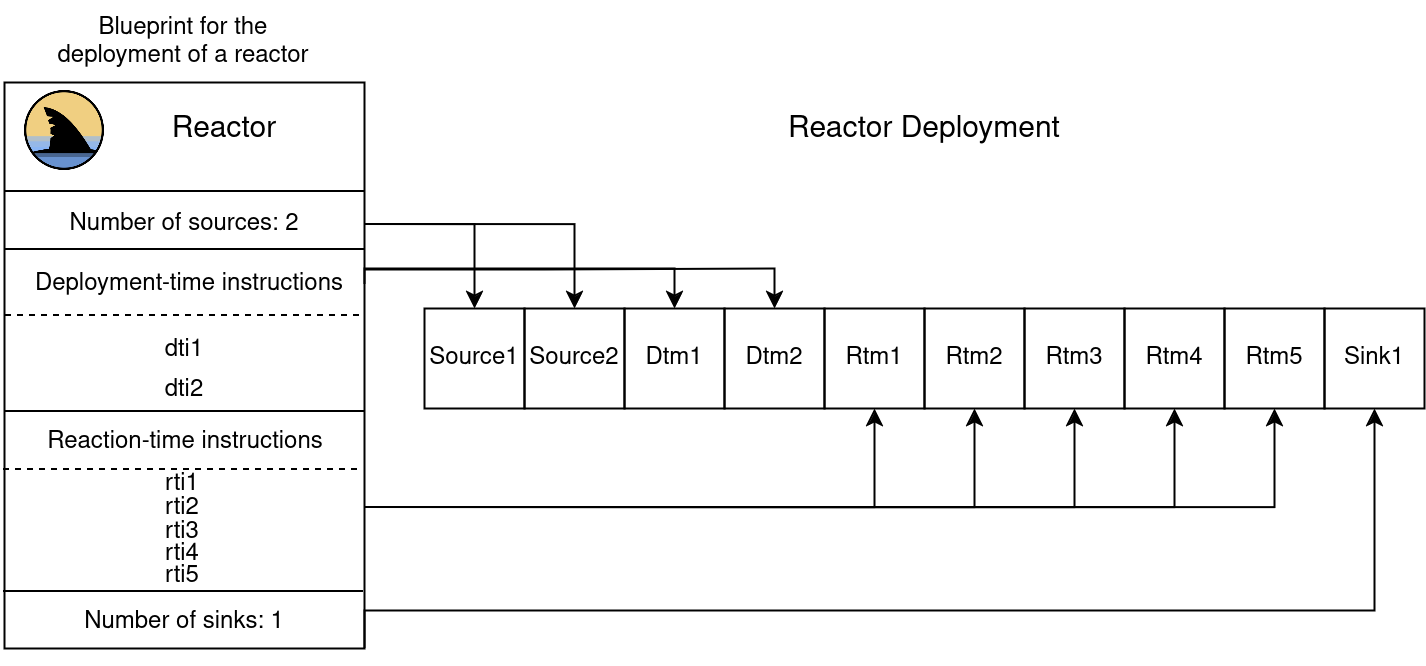
\includegraphics[width=\textwidth]{rd.drawio}
	\caption{Reactor deployment, from blueprint to memory block}
	\label{fig:rde}
\end{figure} 

\subsection{Starting the Deployment}
The deployment of a reactor connects to the runtime in order to communicate with the system. The purely reactive programming language is connected to the 'outside world' with regular Elixir functions that express how the RP receives and sends information for the given domain or use case. Sources are connected to a function that call's the next value for the sources after each iteration of the deployed reactor. Similarly the sinks are connected to a function that given the values of the sink handles them in the way required by the use case. The runtime will, after the deployed reactor reacted, call the function that handles the sinks. When the 'sinks function' terminates the runtime calls the 'sources function', on termination new values are provided to the sources of the deployed reactor and everything iterates on and on for as long the runtime is active. Section \ref{sec:evaluation} presents a musical use case where the values found in the sink serve as values used in OSC messages that are transmitted over the network.


\subsection{Managing the Reactors State}
Managing the state of a reactor is handled by a single actor per reactive program or reactor deployment. This actor is built around the GenServer module in Elixir, a behavior module that provides a generic server implementation. We call this module Memory. Memory serves as a single actor that encapsulates multiple functions designed to respond to various messages or calls. These functions collectively define the behavior of the Memory. One instance of Memory represents the memory block (\ref{fig:rde})of a deployed reactor.
All calls to memory are synchronous this ensures that the values within memory are accessed by only one operation at a time, thereby maintaining the integrity of the memory block.

\chapter{Distribution} \label{sec:distribution}
The cluster environment over which we distribute the first-class reactors is an environment where no communication between reactors (on different nodes) exists. In this thesis we focus on starting  different configurations on different cluster nodes. A configuration exists out of three things. The bytecode for a (composed) reactor, connecting functions for the source and sink and the node(s) on which that configuration should be deployed. 

Technically the cluster is setup on a shared nothing architecture (\cite{DBLP:journals/debu/Stonebraker86}). This allows us to build the cluster environment with independent nodes. Since nothing is shared we can easily add and remove nodes form the cluster environment. This flexibility and modularity allows us to organize different sized cluster environments. A cluster contains a master node and worker nodes. The master node will distribute a configuration to worker nodes. All the nodes in one cluster environment have the same code base (hvm) but do not necessarily run the same composed reactor. The master node can distribute different reactors (represented in byte code) and different connecting functions (represented in Elixir code) based on the specifications in the configuration. The master node contains two libraries. One with all (composed) reactors and a second one with all connecting functions. 

To organize the deployment configurations for a cluster environment we developed a small domain specific language. This allows us to describing the deployed cluster environment in a declarative way. Describing per worker node the composed reactor and connecting functions that have to be send to a specific (group of) node(s).

\section{Multi-Node Deployment Configuration}
The declarative input file we use to distribute the configurations is a yaml file. YAML is a human-readable data serialization language that is often used for writing configuration files. The structure of a YAML file is a map or list that follows a hierarchy based on the indentation. This allows us to define with a declarative syntax and purpose-specific abstractions, how the deployment should take place. By decoupling the configuration from the logic we have a cleaner and more modular codebase. This separation allows non-developers to easily modify configuration settings without delving into the code. For example the use case is a musical instrument where the user is restricted to three things, What data to connect to the input, how to react on the data and what to do with the values leaving the reactors. Documentation is required for the user to know what reactors, connectors and sinks are available for the application domain and how they work.

Listing \ref{code:Yaml} shows a small example, where two deployments are defined with purpose-specific abstractions like task, reactor, node, connector and sinks. This deployment configuration file will start the same reactor p1 with different connector functions in the same cluster environment. Abstraction task and node are linked to the system and not to the application domain. Task can be start, update or stop and node holds the address of the actual node in the cluster environment. Reactor, connector and sinks are the abstractions that come with the domain and will differ according to the use case. 


\begin{lstlisting}[language=C, caption={YAML code}, captionpos=b,label={code:Yaml}, basicstyle=\ttfamily, frame=single]
deployments:
  - task: start
    reactor: p1
    node: node2@0.0.0.0
    connector_1: f1
    connector_2: t2
    sinks: s1
  - task: start
    reactor: p1
    node: node3@0.0.0.0
    connector_1: f3
    connector_2: t1
    sinks: s1
\end{lstlisting}

The YAML file is parsed and validated in the translation process from YAML to Elixir data structure (nested list). For each abstraction in the YAML file a list with valid elements exist and all input will be validated against that list in the translation tool. When the deployment configuration succeeds validation, the translated configuration  information will be transmitted to the distribution module on the master node in the elixir cluster environment. The logic to start all composed reactors in the cluster is written in Elixir and part of the common code base between nodes. 

\begin{figure}[h]
	\centering
	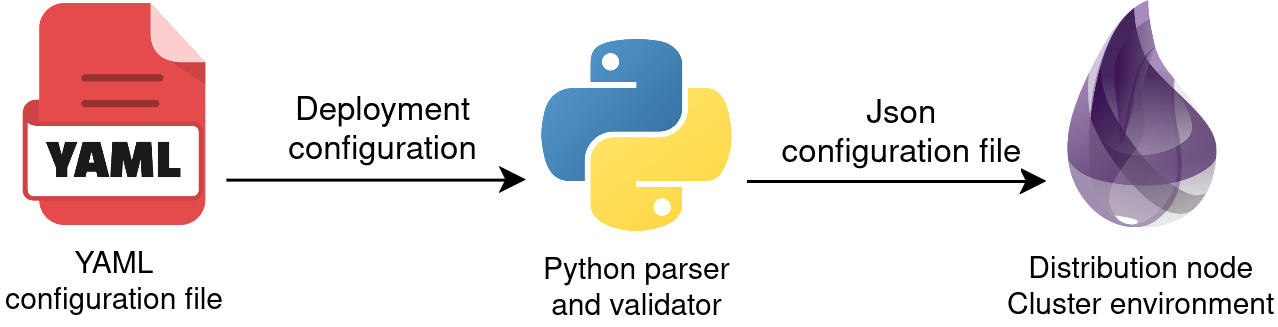
\includegraphics[width=0.8\textwidth]{yaml.drawio}
	\caption{The DSL in YAML is parsed with Python into Elixir's list data structure}
	\label{fig:yaml}
\end{figure}  

Figure \ref{fig:yaml} visualizes the process of sending the configuration file through the Python translation and validation tool. The third step in this visualization represents the interpretation of the Elixir data structure, produced in step 2, by the distribution module on the master node in the cluster environment.


\section{Distributed Hvm}
The distribution module is considered the master of the cluster environment. The cluster is controlled in a centralized way with a master node and worker nodes. The master node controls the deployment of a worker node. The worker node in this setting of reactive programming will not stop working until the master node requires it to stop. Each worker node can be seen as a (composed) reactor.  

Deploying a reactor on the cluster involves sending the bytecode for the requested reactor and the Elixir code for the connecting functions to the Hvm module on the selected node. The ability to send the actual code to deploy a reactor allows us to dynamically alter the cluster environment. At this point no failure detection has been build into the reactors. For now any management of the cluster environment is not part of the reactive program.  

Once the cluster is established, with one master connected to all worker nodes, the reactor or our reactive program is started and will keep on reacting, that is producing sink values based on the sources each iteration of the reactor receives. This setup ensures that the reactive program can respond to changes and maintain operations effectively across the distributed system. Figure \ref{fig:rdi} shows the concept of deploying the reactors from the distribution module into a chosen number of nodes. One reactor can be deployed to an 'unlimited' number of nodes. Each deployment counts as an individual deployment of the configured reactor. 

\begin{figure}[h]
	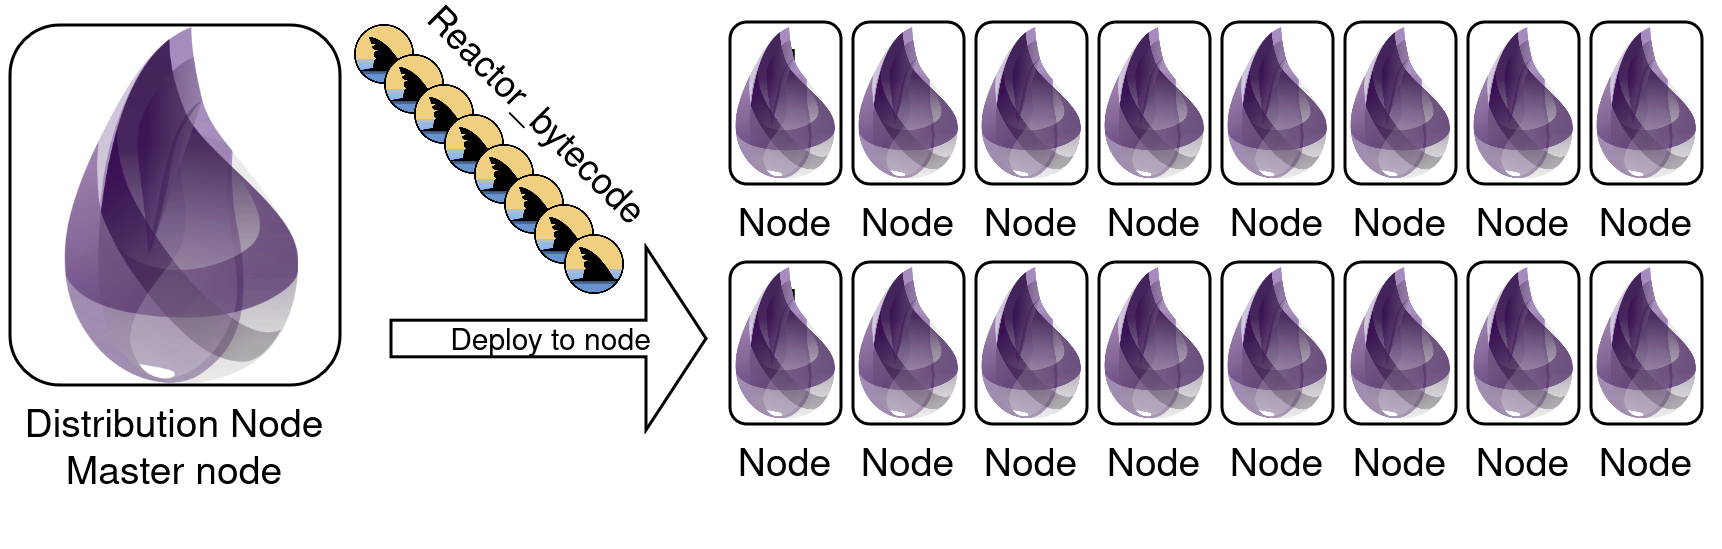
\includegraphics[width=\textwidth]{distribution300.drawio}
	\caption{Distributing reactor deployment on Elixir cluster}
	\label{fig:rdi}
\end{figure}  

\section{Cluster Environment}
The cluster environment of our system is built upon the actor model of computation (\cite{hewitt:hal-01163534}). In this context, actors serve as the fundamental units of the reactive programming environment. The actor model is a mathematical model where actors are universal primitives of computation. Each actor possesses its own state and behavior and communicates with other actors through message passing. This model provides a robust framework for concurrent and distributed systems, ensuring scalability and fault tolerance.

In our cluster environment, actors are the primary entities that facilitate communication and computation. Currently, the communication between actors is confined to individual nodes within the cluster. This design choice simplifies the initial implementation and ensures that each node operates independently, reducing the complexity of inter-node communication.

A worker node in the cluster consists of two primary actors. The first actor is responsible for the process of the hvm, which handles the runtime for deployed reactors. The second actor manages the state, or memory, of the hvm. To ensure the consistency of the hvm's memory, communication between these actors is synchronous. This synchronous communication guarantees that each call to the memory finishes before the next call is accepted, thereby maintaining data integrity and preventing race conditions.

The actor model of Erlang, which our system is inspired by, represents each process as an actor with a mailbox. This model allows for both synchronous and asynchronous communication. Asynchronous communication is particularly advantageous in distributed systems as it enables actors to continue their operations without waiting for responses, thereby improving overall system performance and responsiveness. Future enhancements, such as inter-node communication and leveraging asynchronous messaging, could further improve the system's capabilities.

\chapter{Evaluation} \label{sec:evaluation}


\section{Evaluating the Cluster Environment}

The single master node with a virtually unlimited amount of worker nodes that are all individual from each other gives us a flexible setup to work with. For example, the isolation of failure makes sure that when one node fails for some reason the cluster will not be affected by it. Similarly having the same code base on all nodes helps pointing out eventual problems with worker nodes. From a performance viewpoint the cluster environment is not resource hungry. The number of nodes that simulate the cluster can easily be a tenfold on one machine . The reactors itself have a very light computational cost in the musical use case. The reactors only use some basic arithmetic operations. One Elixir node consumes about 90MB of memory and virtually no processor time when idle and about 3\% when running the use case. This allows to simulate a cluster on one laptop machine with over a hundred nodes. Potentially allowing for big cluster environments on physically spaced machines. In the scope of this work only cluster environments running on one laptop where tested. The size of the cluster was never a problem until the hardware resources of the test machine became the limiting factor around 100 nodes.

In the (next) section \ref{sec:drmg} we present the Distributed reactive melody generator as a use case for the cluster environment. The idea that an unlimited amount of devices (internet of things) generate information that can be reacted on in a way that the information is transformed into synthesized sound. The 'instrument' generates sound on a continuous basis. The sound never stops for as long as the system exists. The artistic idea is somewhat similar to Longplayer, a one-thousand year long composition located at Trinity Buoy Wharf in London (\cite{Longplayer2024}). 

\section{Distributed reactive melody generator} \label{sec:drmg}
For a melody to be generated we need at least one source of information. This source can be manipulated and transferred to the sound server. The maximum number of sources will be defined by the actual system and will depend mainly on the systems hardware constraints (that are expandable). The distributed first-order reactors in the cluster environment provide the sink values to be send to the sound server with the OSC protocol (\cite{schmeder2010best}). The OSC messages are send to a sound server to trigger generation of sound. It is the reactors that, by reacting on incoming streams of data, produce the values that result in a rhythmical flow of OSC messages to the sound server. We have a virtually unlimited amount of information that is reactively transformed in a never ending audible piece of sound.

\begin{figure}[h]
	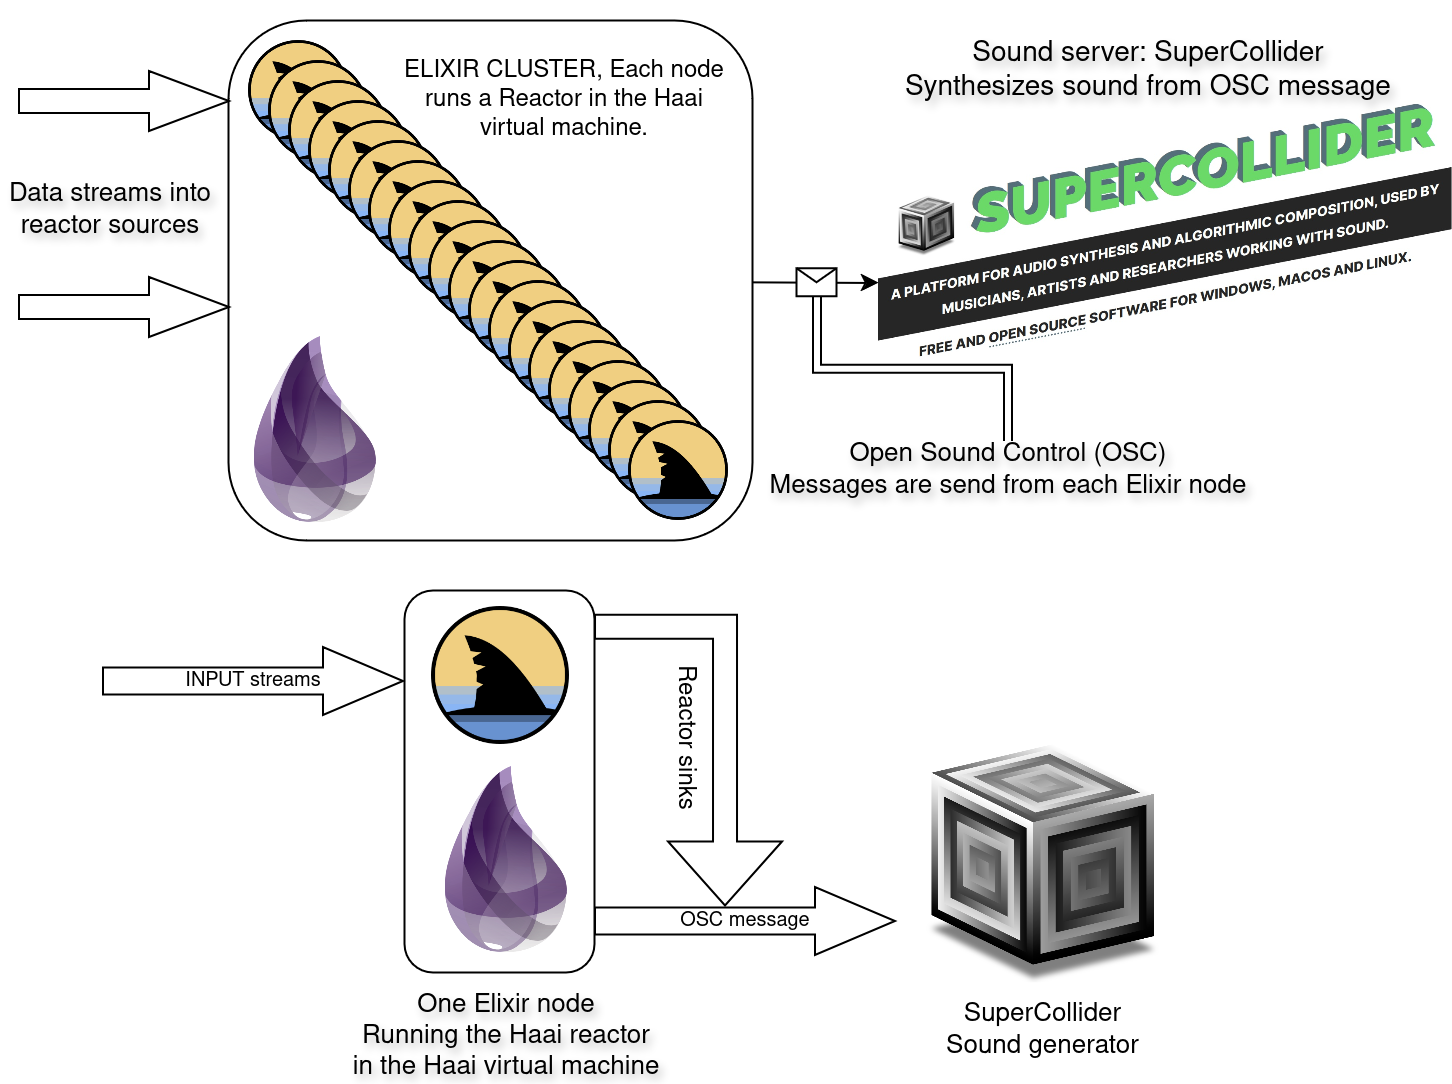
\includegraphics[width=\textwidth]{drmg200.drawio}
	\caption{Distriuted Reactive Melody Generator}
	\label{fig:drmg}
\end{figure}
 
In the current configuration the flow of rhythmical messages is related to the duration of each sound. A reactor will iterate at a varying speed related to the duration of the sound that will be generated form the sink values of that reactor. Each reactor iterates over and over but each iteration has a defined duration, this duration is virtually equal to the duration for a sound calculated by the reactor. A reactor will calculate the new values, sleep for the calculated duration and then provide the new values in the sink. 

\subsection{Sound Server}
The synthesizer that produces the sound is a Synthdef inside the sound server named Supercollider. Supercollider is an open-source platform for audio synthesis and algorithmic composition. Developed by James McCartney in the late 1990s (\cite{scBook}), it has since become a powerful tool in the fields of music technology, computer music, and sound art. Supercollider provides a flexible and expressive environment for creating and manipulating sound in real-time, making it an invaluable resource for both research and artistic exploration. Some main features and usage examples of Supercollider include: Audio Synthesis, Real-time Processing and Algorithmic Composition.

%\begin{description}
%	\item[Audio Synthesis] Supercollider offers a wide range of synthesis techniques, including additive, subtractive, granular, and physical modeling synthesis. Users can create complex sounds by combining these techniques and modulating parameters in real-time.
%	\item[Real-time Processing] One of Supercollider's key strengths is its ability to process audio in real-time. This makes it suitable for live performances, interactive installations, and other time-sensitive applications.
%	\item[Algorithmic Composition] Supercollider provides tools for generating music algorithmically, allowing users to create compositions based on mathematical algorithms, rulesets, or generative processes.
%	\item[Integration with External Hardware] Supercollider can interface with external MIDI controllers, audio interfaces, and other hardware devices, enabling users to incorporate physical instruments and sensors into their sound projects.
%	\item[Community and Documentation] Supercollider has a vibrant online community of users who share code, tutorials, and resources. Additionally, comprehensive documentation is available, including tutorials, reference guides, and examples to help users learn and master the software.
%	\item[Research in Music Technology] Digital signal processing, human-computer interaction, and machine learning for music. Researchers leverage its flexibility and programmability to prototype new algorithms, experiment with novel synthesis techniques, and investigate the perceptual and cognitive aspects of sound.
%	\item[Composition and Sound Design] Supercollider is used to create innovative works that push the boundaries of traditional music and sound art. Its ability to generate complex and evolving textures, as well as its support for algorithmic composition, makes it a valuable tool for exploring new sonic territories.
%	\item[Teaching and Learning] Supercollider is increasingly incorporated into music technology and computer music curricula at universities and colleges worldwide. It provides students with hands-on experience in sound synthesis, programming, and digital audio processing.
%
%\end{description} 
\subsection{Sound Server Communication}
The communication between the nodes in the Elixir cluster and the sound server is done over the network using the UDP network protocol. The sound server can handle a virtual unlimited amount of messages, but is practically bounded to the udp buffer size on the actual machine that runs the sound server. As such the Elixir cluster of reactors can be of any feasible size and the sound server will respond on any number of messages by synthesizing the requested sound. 

\subsection{Musical Values}
The reactor or program that runs on all nodes in the cluster does for each note the following. It calculates two values given two input streams of numbers. The first source is a stream of base frequencies, represented as a float number, the second source is again a stream of numbers representing a tempo in beats per minute (bpm)

\subsubsection*{Consonant notes}
Consonant notes sound harmonious when played together. consonance can be expressed as a ratio between two notes or frequencies. Ratios like the perfect fifth (frequency ratio of 3:2) and the major third (frequency ratio of 5:4) are very commonly used ratios in a musical setting. One of the two reactors in the main program used for this use case calculates such a note for a given base note, both are expressed in there actual frequency represented as a float number.

\subsubsection*{Tempo}
We can express the speed of a musical note progression in beats per minute (bpm). From that number we can then calculate the duration of individual notes in the musical performance. 

We calculate the time in milliseconds. Since one minute is 60000 milliseconds one can calculate the length of a quarter note with \(q = \frac{60000}{bpm}\) with the assumption that we use a 4/4 time signature. From the length of the quarter note it is easy to find other durations. For example, the duration of a halve note is double that of a quarter note or the duration of a eight note is half the time of a quarter note.

One of the two reactors in the main program used for this use case calculates exactly that, the length for a quarter note and improvises a deviser or multiplier to produce some duration. 

%\backmatter
\chapter{Conclusion}

Reactive Programming (RP) has emerged as a powerful paradigm that models data flow as streams of events, enabling systems to react efficiently to changes and events. This document has explored the principles of reactive programming, its applications, and the development of a framework for distributing first-class reactive programs in a cluster environment. The novel reactive language Haai, which operates independently of a base language, addresses key challenges in reactive programming by preventing the base language from interfering with the reactivity of the program.

The Haai virtual machine, implemented in Elixir and leveraging the Erlang Virtual Machine (BEAM), enables the distribution of reactive programs across a cluster. The evaluation of this cluster environment has demonstrated its flexibility, scalability, and fault tolerance, allowing for the simulation of large cluster environments on a single machine. This capability is crucial for developing and testing distributed reactive systems in a controlled setting before deploying them in real-world scenarios.

A practical use case, the distributed reactive melody generator, showcases the framework's application in transforming streams of data into synthesized sound. This use case involves sending network messages to a Supercollider sound server, highlighting the potential of reactive programming in creating innovative and dynamic systems that respond to real-time events. The ability to transform data streams into audible outputs underscores the versatility and creativity that reactive programming can bring to various domains, including music and multimedia.

The canonical reactive program model, exemplified by spreadsheets, demonstrates the power of time-varying values and the propagation of change. The Haai language, with its clear and concise syntax, allows for the creation of complex behaviors from simple building blocks, promoting readability and maintainability. The use of behaviors and events as fundamental abstractions in RP ensures that systems can handle both continuous and discrete changes efficiently.

Overall, this work contributes to the advancement of reactive programming by providing a robust framework for distributed reactive programming and demonstrating its practical applications in a musical context. The Haai language and its virtual machine offer a promising avenue for further research and development in the field of reactive systems. Future work could explore additional use cases, optimize the performance of the Haai virtual machine, inter-connectivity between cluster nodes and investigate the integration of reactive programming with other emerging technologies.

\printbibliography
\end{document}
